\documentclass{beamer}

\usepackage{pscyr}

\usepackage[T2A]{fontenc}
\usepackage[utf8]{inputenc}
\usepackage[english, russian]{babel}

\usepackage{amsmath}
\usepackage{amssymb}
\usepackage{amsthm}
\usepackage{mathrsfs}
\usepackage{bbm}

\usepackage{graphicx}

\title[Биржевые торги с непрерывными ставками]{%
  О модификации многошаговой модели биржевых торгов с непрерывными ставками%
}

\author{%
Пьяных А.И.\\
\texttt{artem.pyanykh@gmail.com}%
}

\institute{%
  Московский Государственный Университет \\
  Факультет вычислительной математики и кибернетики%
}

\date{Ломоносовские чтения. 2016}

\subject{Game theory}

\usetheme{Warsaw}

\DeclareMathOperator{\Ind}{\ensuremath{\mathbbm{1}}}
\DeclareMathOperator{\E}{\ensuremath{\mathbb{E}}}

\newcommand{\Borel}{\ensuremath{\mathscr{B}}}
\newcommand{\Co}{\ensuremath{\beta}}
\newcommand{\Dco}{\ensuremath{\overline{\beta}}}
\newcommand{\di}{\ensuremath{\mathrm{d}}}

\begin{document}

\begin{frame}
  \titlepage
\end{frame}

\begin{frame}
  \frametitle{Содержание}
  \tableofcontents
\end{frame}

\section[]{Краткое описание модели}

\begin{frame}
  \frametitle{Краткое описание}
  \begin{itemize}
  \item Между двумя игроками в течение $n \leqslant \infty$ шагов происходят
    торги за однотипные акции.
  \item Цена акции $s$ определяется ходом случая в соответствии с распределением
    $\mu$.
  \item Игрок 1 (инсайдер) знает цену $s$, игрок 2 знает только вероятностное
    распределение $\mu$.
  \item На каждом шаге $t$ игроки делают ставки. Игрок, предложивший большую
    ставку, покупает у другого акцию. При равных ставках сделка не состоится.
  \end{itemize}
\end{frame}

\section[]{Обзор существующих результатов}

\begin{frame}
  \frametitle{Обзор результатов}
  
  \only<1>{
    \framesubtitle{Модели с непрерывными ставками}
    
    \begin{itemize}
    \item%
      \cite[De Meyer, Saley, 2002]{demeyer02}:
      \begin{itemize}
      \item распределение цены $\mu$ с двухточечным носителем в $\{0, 1\}$,
      \item ставки принимают действительные значения.
      \item цена сделки равна наибольшей предложенной ставке.
      \end{itemize}
      Найдено решение $n$-шаговой игры и асимптотика ликвидной цены акции в
      бесконечной игре.
      
    \item%
      \cite[De Meyer, Saley, 2002]{demeyer02arb}. Обобщение результатов
      \cite{demeyer02} для распределений $\mu$ на $(\mathbb{R},
      \mathscr{B}(\mathbb{R}))$ с конечным мат. ожиданием.
      
    \item%
      \cite[De Meyer, 2010]{demeyer10}. Цена сделки определяется в соответствии
      с механизмом $T$, удовлетворяющим набору условий. Получена асимптотика
      ликвидной цены акции.
    \end{itemize}
    
    В \cite{demeyer10} одно из условий на $T$ --- существование значения в
    $n$-шаговой игре для любого распределения $\mu$.
  }

  \only<2>{
    \framesubtitle{Модели с дискретными ставками}
    
    \begin{itemize}
    \item%
      \cite[Доманский, 2007]{domansky07}:
      \begin{itemize}
      \item распределение $\mu$ с двухточечным носителем в $\{0, m\}$,
      \item ставки принимают целые значения из $\overline{0, m}$,
      \item цена сделки равна наибольшей предложенной ставке.
      \end{itemize}
      
      Найдено решение бесконечно-шаговой игры.

    \item%
      \cite[Доманский, Крепс, 2007]{domansky11}. Обобщение \cite{domansky07} для
      распределений $\mu$ над $\mathbb{Z}_+$ (т.е. цена акции может принимать
      любое целое значение).

    \item%
      \cite[Пьяных, 2016]{pyanykh16}. Если $p_{min}$ и $p_{max}$ --- меньшая и
      большая ставки, то сделка осуществляется по цене 
      \[
        \beta p_{min} + (1-\beta) p_{max}, \, \beta \in [0,1].
      \]
      
      Получено решение бесконечно-шаговой игры с распределением цены $\mu$ с
      двухточечным носителем.
    \end{itemize}
  }
  
  \only<3>{
    Параметр $\beta$ можно интерпретировать как переговорную силу покупателя.
    Такой механизм сделки был рассмотрен в \cite[Chatterjee, 1983]{chatterjee83}
    в контексте двустороннего аукциона с неполной информацией. 

    В \cite[Myerson, 1983]{myerson83} было показано, что при определенных
    условиях $\beta = 1/2$ оптимальная с точки зрения общей полезности. 
    
    Из результатов \cite{pyanykh16} следует, что при $\beta = 1/2$ инсайдер
    получает наименьший выигрыш для любых распределений $\mu$.
    
    В данной работе рассмотрена модификация модели с непрерывными ставками из
    \cite{demeyer02} с использованием вышеописанного механизма проведения
    транзакции. }
\end{frame}

\section[]{Постановка задачи}

\begin{frame}
  \frametitle{Постановка задачи}
  
  \only<1>{
    \begin{itemize}
    \item Пусть $S = \{H, L\}$ --- множество возможных состояний рынка и $s \in
      S$ реальное состояние. В состоянии $H$ цена акции равна $1$, иначе ---
      $0$.
    \item Обозначим $y_t = (y^R_t, y^N_t)$ портфель инсайдера на $t$-м шаге
      торгов, где $y^R_t$ и $y^N_t$ --- количество единиц рискового актива и
      денег соответственно.
    \item Если на $t$-м шаге игроки делают ставки $p_{1,t}, p_{2,t} \in [0,1]$,
      то портфель $y_t$ = $y_{t-1} + t(p_{1,t}, p_{2,t})$, где при $\Dco = 1 - \Co$
      \[
        t(p_1,p_2) =
        \Ind_{p_1 > p_2}(1, -(\Co p_1 + \Dco p_2)) +
        \Ind_{p_1 < p_2}(-1, \Dco p_1 + \Co p_2).
      \]
    \item Стоимость портфеля равна
      \[
        V(y_t) = \Ind_{s = H} y^R_t + y^N_t.
      \]
      Цель игроков --- максимизировать стоимость итогового портфеля $y_n$.
    \end{itemize}

  }
  
  \only<2>{%
    \framesubtitle{Прямая игра}%
    Пусть $h_t = (p_{1,1}, p_{2,1}, \ldots, p_{1,t}, p_{2,t})$ --- история
    ставок к $t$-му ходу, а $H_t$ --- множество всевозможных $h_t$. Также через
    $\Delta(X)$ обозначим совокупность всех распределений на $(X, \Borel(X))$.
    
    \begin{itemize}
    \item%
      Перед началом игры ходом случая выбирается $s \in S$ так что $P(s = H) =
      P, \, P(s = L) = 1-P$.
    \item%
      Стратегией игрока 1 является последовательность ходов $\sigma = (\sigma_1,
      \ldots, \sigma_n)$, где $\sigma_t = (\sigma^H_t, \sigma^L_t)$, и
      $\sigma^s_t: H_{t-1} \rightarrow \Delta([0,1])$.
    \item%
      Стратегией игрока 2 является последовательность ходов $\tau = (\tau_1,
      \ldots, \tau_n)$, где $\tau_t: H_{t-1} \rightarrow \Delta([0,1])$.
    \item%
      Выигрыш первого игрока равен
      \begin{equation*}
        g_n(P, \sigma, \tau) = \E_{P, \sigma, \tau} V(y_n).
      \end{equation*}
    \end{itemize}

  }
  
  \only<3>{%
    \framesubtitle{Прямая игра}%
    Обозначим данную игру $G_n(P)$. Ее верхнее и нижнее значения даются
    формулами
    \begin{equation*}
      V_{1,n}(P) = \sup_\sigma \inf_\tau g_n(P, \sigma, \tau), \:
      V_{2,n}(P) = \inf_\tau \sup_\sigma g_n(P, \sigma, \tau).
    \end{equation*}
    Если $V_{1,n}(P) = V_{2,n}(P) = V_n(P)$ то игра имеет значение $V_n(P)$.

  }
  
  \only<4>{%
    \framesubtitle{Рекурсивная структура прямой игры}

    Представим стратегию игрока 1 в $G_{n+1}(P)$ как $(\sigma_1,
    \tilde{\sigma})$, где $\sigma_1$ --- ход игрока на 1 шаге, а
    $\tilde{\sigma}$ --- стратегия в игре продолжительности $n$, зависящая от
    ставки $p_1$. 

    Аналогично представим стратегию игрока 2 как $(\tau_1, \tilde{\tau})$. 

    Пусть также $P(p_1)$ --- апостериорная вероятность состояния $H$ в
    зависимости от ставки игрока 1.

    \begin{itemize}
    \item Для значения выигрыша справедлива формулами
      \begin{equation*}
        g_{n+1}(P, \sigma, \tau) =
        g_1(P, \sigma_1, \tau_1) +
        \E_{P, \sigma} g_n(P(p_1), \tilde{\sigma}(p_1), \tilde{\tau}(p_1)).
      \end{equation*}

    \item Для нижнего значения игры справедлива формулами
      \begin{equation*}
        V_{1,n+1}(P) \geqslant 
        \sup_{\sigma_1} \inf_{\tau_1} g_1(P, \sigma_1, \tau_1) +
        \E_{P, \sigma} V_{1,n}(P(p_1)).
      \end{equation*}
    \end{itemize}

  }
  
  \only<5>{%
    \framesubtitle{Двойственная игра}
    
    Двойственная игра $G_n^*(x)$ определяется следующим образом.

    \begin{itemize}
    \item Перед началом торгов игрок 1 выбирает $s \in S$. В том случае, если он
      выбрал $H$, то по окончании игры он платит игроку 2 штраф размера $x$.
      Игрок 1 также контролирует значение $P$. В остальном правила двойственной
      игры аналогичны правилам прямой игры.
    \item Функция выигрыша задана как
      \begin{equation*}
        g^*_n(x, (P, \sigma), \tau) = x P - g_n(P, \sigma, \tau).
      \end{equation*}
      Игрок 2 стремиться максимизировать ее значение.
    \end{itemize}

  }
  
  \only<6>{%
    \framesubtitle{Двойственная игра}

    Верхнее и нижнее значение игры $G^*_n(x)$ даются формулами
    \begin{equation*}
      W_{1,n}(x) = \inf_{(P, \sigma)} \sup_\tau g^*_n(x, (P, \sigma), \tau), \:
      W_{2,n}(x) = \sup_\tau \inf_{(P, \sigma)} g^*_n(x, (P, \sigma), \tau).
    \end{equation*}
    Если $W_{1,n}(x) = W_{2,n}(x) = W_n(x)$, то игра имеет значение $W_n(x)$.
  }
  
  \only<7>{%
    \framesubtitle{Рекурсивная структура двойственной игры}

    Для двойственной игры справедлива та же рекурсивная декомпозиция, что и для
    прямой игры. В частности для нижнего значения игры имеет место формула
    \begin{equation*}
      W_{2,n+1}(x) \geqslant \sup_{\tau_1} \inf_{p_1} W_{2,n}(x - g^H_1(p_1,
      \tau_1) + g^L_1(p_1, \tau_1)) - g^L_1(p_1, \tau_1),
    \end{equation*}
    где $g^H(p_1, \tau_1) = g_1(1, p_1, \tau_1)$ и $g^L(p_1, \tau_1) = g_1(0,
    p_1, \tau_1)$.

  }
\end{frame}

\section[]{Анализ прямой и двойственной игр}

\begin{frame}
  \frametitle{Анализ прямой и двойственной игр}
  
  \only<1>{
    Для одношагового выигрыша игрока 1 справедлива формула
    \framesubtitle{Одношаговый выигрыш}
    \begin{multline*}
      g_1(P, \sigma_1, p_2) = P \int_I \biggl[
      \Ind_{p_1 > p_2}(1 - \Co p_1 - \Dco p_2) +
      \Ind_{p_1 < p_2} \times \\
      \times (\Dco p_1 - \Co p_2 - 1)
      \biggr] \; \sigma^H_1(\di p_1)
      + (1-P) \int_I \biggl[
      \Ind_{p_1 > p_2} \times \\
      \times (- \Co p_1 - \Dco p_2)
      + \Ind_{p_1 < p_2}(\Dco p_1 - \Co p_2)
      \biggr] \; \sigma^L_1(\di p_1).
    \end{multline*}

  }
  
  \only<2>{
    \framesubtitle{Одношаговый выигрыш}
    Обозначим $\sigma^M_1(p_1) = P \sigma^H_1(p_1) + (1-P) \sigma^L_1(p_1)$
    маргинальное распределение ставки $p_1$.
  }
  
  \only<2,3>{
    \framesubtitle{Одношаговый выигрыш}
    Справедливо следующее равенство:
    \begin{equation*}
      P(p_1) = P \frac{\di \sigma^H_1}{\di \sigma^L_1}(p_1),
    \end{equation*}
    где $\di \sigma^H_1 / \di \sigma^L_1$ --- производная Радона-Никодима.

  }
  
  \only<3>{%
    \framesubtitle{Одношаговый выигрыш}
    Воспользовавшись им для замены меры в формуле для одношагового выигрыша,
    получим

  }
  
  \only<3,4>{%
    \framesubtitle{Параметризация хода инсайдера}
    \begin{multline*}
      g_1(P, \sigma_1, p_2) =
      \int_I \Ind_{p_1 > p_2} \biggl[
      P(p_1) - \Co p_1 - \Dco p_2
      \biggr] \; \sigma^M_1(\di p_1) \; + \\
      + \int_I \Ind_{p_1 < p_2} \biggl[
      \Dco p_1 + \Co p_2 - P(p_1)
      \biggr] \; \sigma^M_1(\di p_1).
    \end{multline*}

  }
  
  \only<4>{%
    \framesubtitle{Параметризация хода инсайдера}
    Данная формула дает способ параметризации хода игрока 1.
    \begin{itemize}
    \item%
      Возьмем случайную величину $u$, равномерно распределенную на $[0, 1]$.

    \item%
      Пусть $f(\cdot)$ -- левая обратная функции распределения $p_1$. При этом
      $f(u)$ и $p_1$ одинаково распределены. 

    \item%
      Пусть $Q(u) = P(f(u))$.
    \end{itemize}


  }
  
  \only<5>{%
    \framesubtitle{Параметризация хода инсайдера}
    Функции $f$ и $Q$ должны удовлетворять следующим свойствам, чтобы служить
    параметризацией некоторого хода $\sigma_1$ игрока 1:
    \begin{enumerate}
    \item $f$ не убывает на $[0, 1]$,
    \item $\int_0^1 Q(u) \di u = P$,
    \item $\forall u_1, u_2 \in [0, 1]: f(u_1) = f(u_2) \implies Q(u_1) = Q(u_2)$.
    \end{enumerate}
  }
  
  \only<6>{%
    \framesubtitle{Оценка выигрыша игрока 1 в игре $G_{n+1}(P)$}
    
    Оценка выигрыша в терминах $f$ и $Q$ дается формулой
    \begin{multline*}
      \int_0^1 \Ind_{f(u) > p_2} (Q(u) - \Co f(u) - \Dco p_2) \di u \enskip + \\
      + \int_0^1 \Ind_{f(u) < p_2} (\Dco f(u) + \Co p_2 - Q(u)) \di u \;
      + \int_0^1 V_{1,n}(Q(u)) \di u.
    \end{multline*}
  }
  
  \only<7>{%
    \framesubtitle{Параметризация хода неосведомленного игрока}
    Аналогично проводится параметризация хода игрока 2 в двойственной игре.
    \begin{itemize}
    \item%
      Возьмем случайную величину $u$, равномерно распределенную на $[0, 1]$.

    \item%
      Пусть $h(\cdot)$ -- левая обратная функции распределения $p_2$. При этом
      $h(u)$ и $p_2$ одинаково распределены. 
    \end{itemize}

  }
  
  \only<8>{%
    \framesubtitle{Оценка выигрыша игрока 2 в игре $G^*_{n+1}(P)$}

    Оценка выигрыша в терминах $h$ дается формулой
    \begin{multline*}
      W_{2,n}\left(
        x - \int_0^1\left[ \Ind_{h(u) < p_1} - \Ind_{h(u) > p_1} \right] \di u
      \right) \; - \\
      - \int_0^1 \left[
        \Ind_{h(u) < p_1} (-\Co p_1 - \Dco h(u)) +
        \Ind_{h(u) > p_1} (\Dco p_1 + \Co h(u))
      \right] \di u.
    \end{multline*}
  }
  
  \only<9>{%
    Следуя схеме, приведенной в \cite[De Meyer, 2002]{demeyer02}:
    \begin{itemize}
    \item найдены функции $f, Q$, выравнивающие выигрыш инсайдера при $p_2 \in
      [f(0), f(1)]$ в прямой игре;
    \item найдена функция $h$, выравнивающая выигрыш игрока 2 при $p_1 \in
      [h(0), h(1)]$ в двойственной игре;
    \item из соотношений двойственности между верхними и нижними значениями
      прямой и двойственной игр показано, что данные стратегии оптимальны.
    \end{itemize}
    
  }

\end{frame}

\section[]{Результаты}

\begin{frame}
  \frametitle{Результаты}
  
  \only<1>{%
    Значение двойственной игры $G^*_n(x)$ дается формулой:
    \begin{equation*}
      W_{n+1}(x) = \int_0^1 W_n(x - 2u + 1), \, W_0(x) = \min(x, 0).
    \end{equation*}
    
    \begin{figure}[H!]
      \centering
      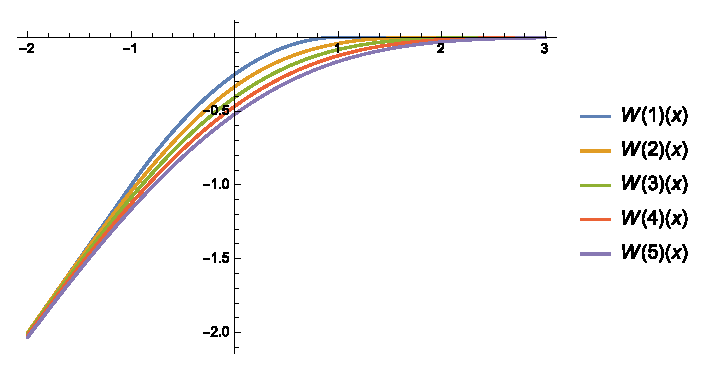
\includegraphics[width=\textwidth]{slides/wGraphs.eps}
    \end{figure}
  }
  
  \only<2>{%
    Значение прямой игры $G_n(P)$ дается формулой:
    \begin{equation*}
      V_n(P) = W_n^*(P),
    \end{equation*}
    где $W^*(P) = \inf_x x P - W_n(x)$ --- сопряженная в смысле Фенхеля функция.

    \begin{figure}[H!]
      \centering
      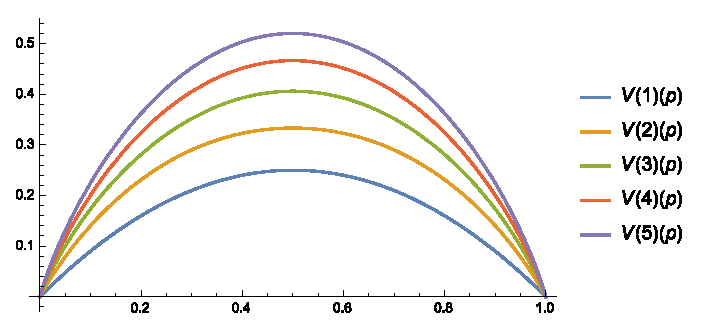
\includegraphics[width=\textwidth]{slides/vGraphs.eps}
    \end{figure}
  }
  
  \only<3>{%
    Функция $Q(u)$ определяется как
    \begin{equation*}
      Q(u) = W'_n(x + 1 - 2u),
    \end{equation*}
    где параметр двойственной игры $x$ удовлетворяет уравнению 
    \begin{equation*}
      W'_n(x) = P.
    \end{equation*}

    \begin{figure}[H!]
      \centering
      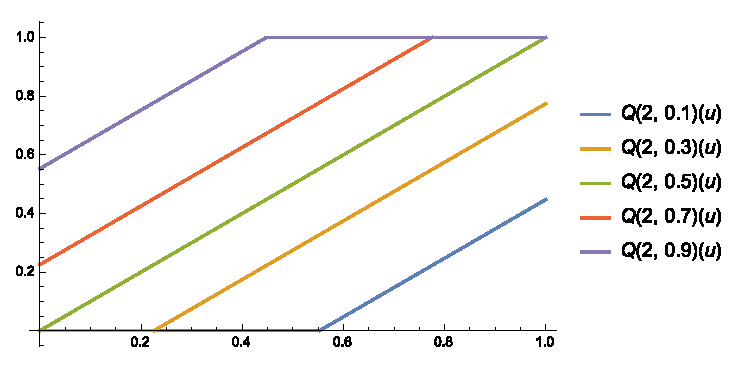
\includegraphics[width=\textwidth]{slides/qGraphs.eps}
    \end{figure}
  }
  
  \only<4>{%
    Функция $f(u)$ определяется как
    \begin{equation*}
      f(u) = 2 (u - 1 + \beta)^{-2} \int_{1-\beta}^u (x - 1 + \beta) Q(x) \di x.
    \end{equation*}
    
    При этом $h(u) = f(u)$.

    \begin{figure}[H!]
      \centering
      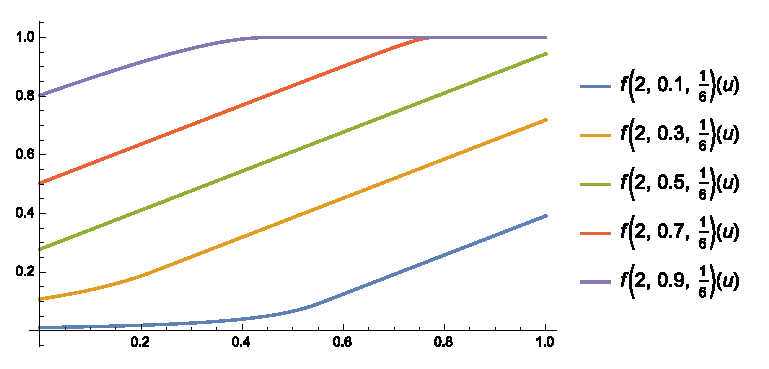
\includegraphics[width=\textwidth]{slides/fGraphs.eps}
    \end{figure}
  }
  
  \only<5>{%
    Сравнивая полученные результаты с существующими, получаем:
    \begin{itemize}
    \item Введение механизма заключения сделки с параметром $\beta$ влияет на
      оптимальные стратегии инсайдера и неосведомленного игрока.
    \item При этом значение игры не зависит от значения $\beta$ и совпадает с
      таковым в \cite[De Meyer, 2002]{demeyer02}. В этом смысле непрерывная
      модель отличается от дискретной \cite[Пьяных, 2016]{pyanykh16}, в которой
      и стратегии и значение игры зависят от значения $\beta$.
    \end{itemize}
  }
\end{frame}

\begin{thebibliography}{99}
\bibitem{demeyer02}
  De Meyer B., Saley H. \emph{On the strategic origin of Brownian motion in
    finance} // Int J Game Theory. 2002.
 
\bibitem{demeyer02arb}%
  De Meyer B., Saley H. \emph{A model of game with a continuum of states of
    nature} // Pr\'{e}publication de l’Institut Elie Cartan, Nancy. 2002.
  
\bibitem{demeyer10}%
  De Meyer B. \emph{Price dynamics on a stock market with asymmetric
    information} // Games and Economic Behavior. 2010.
  
\bibitem{domansky07}%
  Domansky V. \emph{Repeated games with asymmetric information and random price
  fluctuation at finance markets} // Int J Game Theory. 2007.

\bibitem{domansky11}%
  Доманский В.К, Крепс В.Л. \emph{Теоретико игровая модель биржевых торгов:
    стратегические аспекты формирования цен на фондовых рынках} // Журнал Новой
  экономический ассоциации. 2011

\bibitem{pyanykh16}%
  Пьяных А.И. \emph{Многошаговая модель биржевых торгов с асимметричной
    информацией и элементами переговоров} // Вестн. Моск. ун-та. Сер. 15. 2016.
  
\bibitem{chatterjee83}%
  Chatterjee K., Samuelson W. \emph{Bargaining under Incomplete Information} //
  Operations Research, 1983.
  
\bibitem{myerson83}%
  Myerson R., Satterthwaite M. \emph{Efficient Mechanisms for Bilateral Trading}
  // Journal of Economic Theory, 1983.

\end{thebibliography}

\end{document}
